\section{Discussion}
As expected the values for $k_{trap,x}$ and $k_{trap,y}$ increase with an increasing laser power. For the second data set, a reasonable fit can be made using the theoretical relation between $P$ and $k_{trap}$. The fit does however not fit the errors. Therefore one could doubt the accuracy of the result for the corresponding $\alpha$. For the first data set we find that the data does not match the theoretical direct proportionality between $P$ and $k_{trap}$. This seems to be the result of a failing MATLAB code which does not follow the bead. This seems to be caused by other particles in the image  which were not trapped but clearly visible. This could have thrown off the program. Studying the images also reveals that the bead makes some large jumps possibly caused by vibrations of the experimental set-up during the experiment.  \
\begin{wrapfigure}{r}{0.4\textwidth}
    \centering
    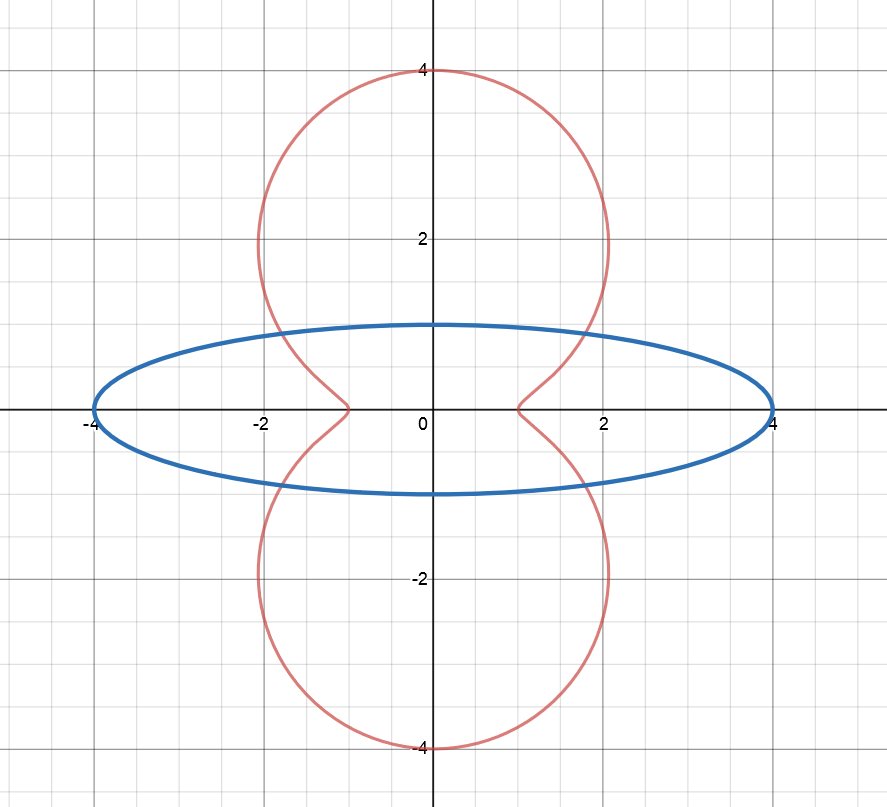
\includegraphics[width=0.35\textwidth,keepaspectratio]{figures/ellipse_inverse.png}
    \caption{An ellipse (blue) and the inverse of its radius (red).}
    \label{fig_ellipse_inverse}
\end{wrapfigure}
The practical manual asks for a calculation of the average trap constant. It was proposed to calculate this as follows: $k_{trap,tot} = \sqrt{k_{trap,x}^2 + k_{Trap,y}^2}$. This would however give inaccurate results since the orientation and shape of the variance is not taken into account. For the calculation of the trap constant we take the inverse of the variance. As explained in the theory we expect the variance to be ellips shaped. However, if we take the inverse of the radius of an ellipse we get a complicated shape such as in figure \ref{fig_ellipse_inverse}. Comparing the shape to a circle with radius $\sqrt{k_{trap,x}^2 + k_{Trap,y}^2}$ shows that the proposed method for the calculation is nonsense. The method described in section \ref{trap_constant} could provide more accurate results. \\
The results for the semi-major and semi-minor axis of the covariance ellipse indicates a inverse correlation of the axis length to the laser power. This is expected given equation \ref{eq_k_trap} and the direct proportionality between the trap constant and laser power. It is interesting that the values for $a$ and $b$ for the first data set seem to have more than a factor 5 difference which would indicate an elongated covariance ellipse. Comparing this to the MATLAB results, there seems to be virtually no difference between $k_{trap,x}$ and $k_{trap,y}$ (only taking into account correct measurements). This points out that the MATLAB algorithm, only projecting the positions on two axis, fails to incorporate the shape of the variance (see figure \ref{fig_ellipse}). Therefore, the method as outlined in section \ref{trap_constant} seems to be promising for calculation of trap constants in any direction independent of the orientation and shape of the trap. \\
The task of recreating a MATLAB script in Python was partially successful. The symmetry centre finding function was successfully implemented as well as the subpixel interpolation function. Due to some dissimilarities in the way MATLAB and Python functions interpolate an unstructured set of data we were unable to get the main tracking function to work. The resulting estimates of the symmetry centre location were not far of but were not dead-on either. \\
Although the MATLAB code works fine in many cases, it showed that it does not always work well. Moreover, for students, the code is long and involves some complicated steps. For these reasons we would suggest using the trackpy for particle tracking. This function shows promising results in speed and accuracy. By visual inspection it is clear that this function had no trouble whatsoever with the data covered in this report. The down side is, although there is elaborated documentation of the function, the maths used for the tracking is not explicitly noted. Therefore students would perhaps have less insight in the tracking mechanism. More information about the trackpy function can be found in the appendix.
